\documentclass[12pt,a4paper]{article}
\usepackage{array}

\usepackage{geometry}
\usepackage{graphicx}
\usepackage{fancyhdr}
\usepackage{amsmath}
\usepackage{amsfonts}
\usepackage{amssymb}
\usepackage{color}
\usepackage{hyperref}
\usepackage{tikz}
\usetikzlibrary{shapes.geometric,arrows,positioning,shadows}
\usepackage{pgfgantt}
\usepackage{float}
\usepackage{listings}
\usepackage{xcolor}
\usepackage{booktabs}
\usepackage{multirow}
\usepackage{array}
\usepackage{subcaption}
\usepackage{titlesec}
\usepackage{multicol}
\usepackage{caption}
\usepackage{colortbl}
\usepackage{xcolor}
\usepackage{multirow}
\usepackage{array}

% Remove color styling that causes table issues
% Professional caption configuration - coordinated styling
\captionsetup{
    font={bf,small},
    textfont={color=bodytext},
    labelfont={color=primaryblue, bf},
    justification=centering,
    singlelinecheck=false,
    labelsep=period,
    skip=10pt,
    position=bottom
}

% Professional subcaption formatting - coordinated styling
\captionsetup[sub]{
    font={bf,footnotesize},
    textfont={color=bodytext},
    labelfont={color=secondaryblue, bf},
    justification=centering,
    singlelinecheck=false,
    labelsep=period,
    skip=8pt
}

% Professional table formatting with coordinated styling
\definecolor{tableheader}{RGB}{0,82,165}         % Primary blue for headers
\definecolor{tablebody}{RGB}{240,248,255}        % Very light blue
\definecolor{tableaccent}{RGB}{25,118,210}       % Secondary blue accent
\definecolor{tableborder}{RGB}{0,82,165}         % Primary blue border

% Additional color definitions for enhanced tables
\definecolor{headertext}{RGB}{255,255,255}       % White text for headers
\definecolor{bodytext}{RGB}{66,66,66}            % Professional dark gray
\definecolor{tablealt1}{RGB}{248,251,255}        % Alternating row color 1
\definecolor{tablealt2}{RGB}{235,245,251}        % Alternating row color 2
\definecolor{greentable}{RGB}{76,175,80}         % Professional green
\definecolor{orangetable}{RGB}{255,152,0}        % Professional orange
\definecolor{purpletable}{RGB}{156,39,176}       % Professional purple

% Enhanced table styling commands
\newcommand{\tableheaderrow}[1]{\rowcolor{tableheader}\textcolor{headertext}{\textbf{#1}}}
\newcommand{\tablealtrow}{\rowcolor{tablealt1}}
\newcommand{\tablealtrowtwo}{\rowcolor{tablealt2}}
\newcommand{\specialheader}[2]{\rowcolor{#1}\textcolor{headertext}{\textbf{#2}}}

% Set default array rule width for professional borders
\setlength{\arrayrulewidth}{1.2pt}

% Configure hyperref with professional colors
\hypersetup{
    colorlinks=true,
    linkcolor=primaryblue,
    filecolor=secondaryblue,      
    urlcolor=accentblue,
    pdftitle={Chapter 1: Introduction to Systems - Code Studio Software Company},
    pdfauthor={Sajidur Rahman Tarafder},
    pdfsubject={Systems Analysis and Design Lab Report}
}

% Enhanced code listings with professional colors
\lstset{
    basicstyle=\ttfamily\footnotesize,
    backgroundcolor=\color{lightgray},
    frame=leftline,
    framerule=3pt,
    rulecolor=\color{primaryblue},
    breaklines=true,
    captionpos=b,
    numbers=left,
    numberstyle=\tiny\color{darkgray}\bfseries,
    stepnumber=1,
    numbersep=12pt,
    keywordstyle=\color{primaryblue}\bfseries,
    commentstyle=\color{mediumgray}\itshape,
    stringstyle=\color{secondaryblue},
    emphstyle=\color{accentblue}\bfseries,
    showstringspaces=false,
    tabsize=2,
    xleftmargin=20pt,
    framexleftmargin=15pt,
    numberbychapter=false,
    firstnumber=1
}

% ===================== PROFESSIONAL COLOR SCHEME =====================
% Define professional color palette
\definecolor{primaryblue}{RGB}{0,82,165}        % Deep professional blue
\definecolor{secondaryblue}{RGB}{25,118,210}    % Medium blue
\definecolor{accentblue}{RGB}{100,181,246}      % Light blue accent
\definecolor{lightblue}{RGB}{173,216,230}       % Light blue for backgrounds
\definecolor{darkgray}{RGB}{66,66,66}           % Professional dark gray
\definecolor{mediumgray}{RGB}{117,117,117}      % Medium gray
\definecolor{lightgray}{RGB}{238,238,238}       % Light gray for backgrounds

% Professional section formatting with modern styling
\titleformat{\section}[hang]
{\normalfont\LARGE\bfseries\color{primaryblue}}
{\colorbox{primaryblue}{\makebox[1.8em]{\textcolor{white}{\thesection}}}~}{0.5em}
{}
[\vspace{2pt}{\color{primaryblue}\hrule height 1pt width \textwidth}]
\titlespacing*{\section}{0pt}{25pt}{18pt}

% Professional subsection formatting with perfect left alignment
\titleformat{\subsection}[block]
{\normalfont\Large\bfseries\color{secondaryblue}}
{\thesubsection.~}{0pt}
{}
[\vspace{1pt}{\color{secondaryblue}\hrule height 0.8pt width \textwidth}]
\titlespacing*{\subsection}{0pt}{20pt}{14pt}

% Modern subsubsection formatting with perfect left alignment
\titleformat{\subsubsection}[block]
{\normalfont\large\bfseries\color{accentblue}}
{\thesubsubsection.~}{0pt}
{}
[\vspace{0.5pt}{\color{accentblue}\hrule height 0.5pt width \textwidth}]
\titlespacing*{\subsubsection}{0pt}{15pt}{10pt}

% Define custom project title formatting (left-aligned with consistent underlines)
\newcommand{\projecttitle}[1]{%
    \vspace{15pt}%
    \noindent{\normalfont\Large\bfseries\color{accentblue}#1}%
    \vspace{1pt}\noindent{\color{accentblue}\hrule height 0.8pt width \textwidth}%
    \vspace{10pt}%
}

% ===================== PROFESSIONAL HEADER SETUP =====================
% Configure geometry for header space
\geometry{
    top=2.5cm,
    bottom=2.5cm,
    left=2.5cm,
    right=2.5cm,
    headheight=25pt,
    headsep=30pt
}

% Professional header and footer design
\fancypagestyle{reportstyle}{%
    \fancyhf{}% Clear all headers and footers
    
    % Header setup
    \fancyhead[L]{\textcolor{primaryblue}{\textbf{CSE 4110 - Systems Analysis \& Design}}}
    \fancyhead[R]{\textcolor{primaryblue}{\textbf{Code Studio Software Company}}}
    
    % Header line
    \renewcommand{\headrulewidth}{1pt}
    \renewcommand{\headrule}{\hbox to\headwidth{%
        \color{primaryblue}\leaders\hrule height \headrulewidth\hfill}}
    
    % Footer setup - only page number
    \fancyfoot[C]{\textcolor{primaryblue}{\textbf{\thepage}}}
    
    % No footer line
    \renewcommand{\footrulewidth}{0pt}
}

% Chapter 2 page style
\fancypagestyle{chapter2style}{%
    \fancyhf{}
    
    % Header setup
    \fancyhead[L]{\textcolor{primaryblue}{\textbf{CSE 4110 - Systems Analysis \& Design}}}
    \fancyhead[R]{\textcolor{primaryblue}{\textbf{Code Studio Software Company}}}
    
    % Header line
    \renewcommand{\headrulewidth}{1pt}
    \renewcommand{\headrule}{\hbox to\headwidth{%
        \color{primaryblue}\leaders\hrule height \headrulewidth\hfill}}
    
    % Footer setup - only page number
    \fancyfoot[C]{\textcolor{primaryblue}{\textbf{\thepage}}}
    
    % No footer line
    \renewcommand{\footrulewidth}{0pt}
}

% Chapter 3 page style
\fancypagestyle{chapter3style}{%
    \fancyhf{}
    
    % Header setup
    \fancyhead[L]{\textcolor{primaryblue}{\textbf{CSE 4110 - Systems Analysis \& Design}}}
    \fancyhead[R]{\textcolor{primaryblue}{\textbf{Code Studio Software Company}}}
    
    % Header line
    \renewcommand{\headrulewidth}{1pt}
    \renewcommand{\headrule}{\hbox to\headwidth{%
        \color{primaryblue}\leaders\hrule height \headrulewidth\hfill}}
    
    % Footer setup - only page number
    \fancyfoot[C]{\textcolor{primaryblue}{\textbf{\thepage}}}
    
    % No footer line
    \renewcommand{\footrulewidth}{0pt}
}

% Title page style (no header/footer)
\fancypagestyle{titlepage}{%
    \fancyhf{}%
    \renewcommand{\headrulewidth}{0pt}%
    \renewcommand{\footrulewidth}{0pt}%
}

% Set default page style after title page
% ===================== ENHANCED STYLING =====================

\begin{document}

% ===================== COVER PAGE =====================

\begin{titlepage}
    \thispagestyle{empty}
    \centering
    \vspace*{0.5cm}
    
    % University motto
    {\large \textbf{"Heaven's Light is Our Guide"}}\\[0.3cm]
    
    % University logo
    \includegraphics[width=3cm]{ruet_logo.png} \\[0.4cm]
    
    % University name

    {\Large \textbf{Department of Computer Science \& Engineering}}\\[0.3cm]
    {\large \textbf{Rajshahi University of Engineering \& Technology}}\\[0.8cm]

    \vspace{0.8cm}
    % Report title
    {\LARGE \textbf{Lab Report-1}}\\[0.2cm]

    \vspace{0.8cm}
    % Course details
    {\Large \textbf{Course Code: CSE 4110}}\\[0.2cm]
    \vspace{0.3cm}
    {\Large \textbf{Course Title: Information Systems Analysis and}}\\
    \vspace{0.3cm}
    {\Large \hspace{-1.0cm}\textbf{Design Sessional}}\\[0.8cm]
    
    
    % Submission details table with proper formatting
    \begin{table}[h!]
    \centering
    \setlength{\arrayrulewidth}{1.5pt}
    \renewcommand{\arraystretch}{1.3}
    \begin{tabular}{|p{7.5cm}|p{7.5cm}|}
        \hline
        \multicolumn{1}{|c|}{\large \textbf{Submitted By:}} & \multicolumn{1}{c|}{\large \textbf{Submitted To:}} \\
        \hline
        \large \textbf{1. Puja Saha} & \multirow{10}{*}{\parbox{7.5cm}{\centering 
        \large \textbf{Emrana Kabir Hashi} \\ 
        \vspace{0.1cm}
        \textbf{Assistant Professor} \\ 
        \vspace{0.1cm}
        \textbf{Department of CSE, RUET}}} \\
        \large \quad \textbf{\hspace{0.2cm}Roll: 2003151} & \\
        \large \quad \textbf{\hspace{0.2cm}Department of CSE, RUET} & \\
        \cline{1-1}
        \large \textbf{2. Md. Rezanur Akndo Riyad} & \\
        \large \quad \textbf{\hspace{0.2cm}Roll: 2003152} & \\
        \large \quad \textbf{\hspace{0.2cm}Department of CSE, RUET} & \\
        \cline{1-1}
        \large \textbf{3. Anika Hossain} & \\
        \large \quad \textbf{\hspace{0.2cm}Roll: 2003153} & \\
        \large \quad \textbf{\hspace{0.2cm}Department of CSE, RUET} & \\
        \cline{1-1}
        \large \textbf{4. Sajidur Rahman Tarafder} & \\
        \large \quad \textbf{\hspace{0.2cm}Roll: 2003154} & \\
        \large \quad \textbf{\hspace{0.2cm}Department of CSE, RUET} & \\
        \hline
        
    \end{tabular}
    \end{table}
    
    \vspace{0.5cm}

\end{titlepage}

% Set page style for the rest of the document
\pagestyle{reportstyle}
\newpage

% ===================== TABLE OF CONTENTS =====================
\renewcommand{\contentsname}{Table of Contents}
\tableofcontents
\newpage

% ===================== MAIN CONTENT =====================

\section{Chapter 1: Introduction to Systems}

\vspace{0.2cm}

\subsection{What is a System?}

In today's interconnected world, systems are fundamental building blocks that shape how we work, communicate, and solve problems. A system can be understood as an organized collection of interrelated components that work together toward achieving a common goal or purpose. These components take inputs from their environment, process them through various operations, and produce meaningful outputs.

Systems are everywhere around us – from the smartphone in our pocket to the complex networks that power the internet. In the business world, organizations rely on various systems to manage their operations, serve customers, and drive growth. Code Studio Software Company exemplifies how a well-designed system can transform business ideas into successful digital solutions.

\subsection{Code Studio Software Company}

In January 2019, Code Studio has emerged as a dynamic software development company that bridges the gap between innovative ideas and digital reality. Originally starting as "Code Art" through the inspiration of friends who shared a passion for technology, the company has evolved into a trusted partner for businesses and startups worldwide.

Based in Rajshahi, Bangladesh, with strategic operations extending to New York, USA, Code Studio has successfully collaborated with over 25 startup companies across different continents. What sets the company apart is its commitment to transforming entrepreneurial visions into tangible digital solutions that users love and businesses depend on.

\subsubsection{Services Offered}

Code Studio's expertise spans across multiple domains of software development, offering comprehensive solutions that cater to diverse business needs:

\begin{itemize}
    \item \textbf{Mobile App Development:} Creating intuitive iOS and Android applications that serve various industries including e-commerce, healthcare, agriculture, and emerging startups. Each app is crafted with user experience at its core.
    
    \item \textbf{Website Development:} Building responsive, secure, and SEO-optimized websites that not only look great but also perform exceptionally well across all devices and search engines.
    
    \item \textbf{UI/UX Design:} Designing user interfaces that are not just visually appealing but also enhance user engagement and drive meaningful interactions between businesses and their customers.
    
    \item \textbf{Machine Learning Solutions:} Developing AI-powered applications and intelligent systems that help businesses leverage data for better decision-making and automated processes.
    
    \item \textbf{Digital Marketing:} Providing comprehensive strategies to optimize online presence and help businesses reach their target audiences more effectively.
    
    \item \textbf{IT Support:} Offering round-the-clock technical assistance and consultation, ensuring that clients can always reach out when they need help or guidance.
\end{itemize}

\begin{figure}[H]
    \centering
    \includegraphics[width=0.8\textwidth]{code_studio_services.png}
    \caption{Services Provided By Code Studio}
    \label{fig:services_overview}
\end{figure}

\subsection{Vision and Mission}

\subsubsection{Vision}
Code Studio's vision is to operate as a fully remote-based company that spreads new ideas across the country to develop new innovations. The company envisions becoming a globally recognized software development organization that leverages cutting-edge mobile and web technologies to transform business concepts into revolutionary digital solutions, while maintaining complete operational flexibility in terms of location, financial management, and time freedom.

\subsubsection{Mission}
Our mission is to focus entirely on mobile app and website development, especially developing new idea-based applications depending on user needs and unique ideas that are shared with us. We are committed to building high-quality, responsive, and secure software solutions while expanding our team size and transitioning to fully remote operations. Through our comprehensive services including digital marketing, video editing, and graphic design, we strive to be the trusted technology partner that delivers innovative solutions with the goal of achieving less investment and more benefit for both our company and our clients.


\subsection{System Characteristics}

Code Studio operates as an open-ended deterministic system with the following key characteristics:

\begin{itemize}
    \item \textbf{Organization:} Structured hierarchical arrangement with CEO leading specialized teams (5 mobile, 7 backend, 2 UI/UX developers)
    \item \textbf{Interaction:} Seamless communication between teams using Google Meet, multi-channel client engagement, technology stack integration
    \item \textbf{Interdependence:} Backend development depends on UI/UX designs, mobile apps rely on backend APIs, coordinated team workflows
    \item \textbf{Integration:} Flutter, React.js, Node.js, and MySQL technologies work together for comprehensive solutions
    \item \textbf{Goal-Oriented:} Primary objective of 98.5\% project success rate, innovation, and client satisfaction
    \item \textbf{Feedback Mechanism:} Client reviews, performance monitoring, and continuous process improvement
\end{itemize}

\subsection{System Components}

The Code Studio system consists of several interconnected components:

\begin{itemize}
    \item \textbf{Input:} Client requirements, business ideas, technical specifications, design assets, budget and timeline constraints
    \item \textbf{Process:} Requirements analysis, UI/UX development, software development (mobile/web), quality assurance, project management
    \item \textbf{Output:} Mobile applications (Flutter), web applications (React.js/Next.js), backend systems (Node.js/MySQL), documentation, support services
    \item \textbf{Control:} Quality control mechanisms, project management controls, security measures, performance monitoring, client approval processes
    \item \textbf{Feedback:} Client feedback systems, performance analytics, market response data, internal process improvement, technical metrics
    \item \textbf{Environment:} Market conditions, regulatory environment, technological landscape, economic factors, competitive landscape
    \item \textbf{Boundary:} Service scope definition, technical boundaries, geographic limits, resource constraints, timeline and budget boundaries
\end{itemize}
\end{itemize}

\subsection{System Type Analysis}

Code Studio operates as an Open-Ended Deterministic System with the following characteristics:

\begin{itemize}
    \item \textbf{Deterministic Aspects:}
    \begin{itemize}
        \item Follows structured development methodologies
        \item Maintains consistent quality standards (98.5\% success rate)
        \item Uses established technology stacks and proven frameworks
        \item Implements predictable project timelines and deliverables
    \end{itemize}
    
    \item \textbf{Open-Ended Features:}
    \begin{itemize}
        \item Continuously evolves with new technologies and client needs
        \item Adapts to different industry sectors (e-commerce, healthcare, education, agriculture)
        \item Scales operations based on project demands (currently handling 20+ concurrent projects)
        \item Remains flexible to changing market requirements and technological advances
    \end{itemize}
\end{itemize}

\subsection{Project Portfolio}

\subsubsection{Project Portfolio Overview}
Code Studio has successfully completed over 90 projects since its inception in January 2019, with 15+ currently running projects. Their portfolio spans across multiple sectors:

\begin{itemize}
    \item \textbf{E-Commerce Applications:} Mobile and web applications that allow users to browse products, make purchases, track orders, and receive personalized recommendations
    
    \item \textbf{Healthcare Solutions:} Telemedicine applications, patient management systems, health tracking apps, and fitness applications offering virtual consultations and electronic health records
    
    \item \textbf{Educational Platforms:} E-learning platforms, language learning tools, educational games, and classroom management systems
    
    \item \textbf{Travel Applications:} Comprehensive travel apps providing functionalities for booking flights, hotels, rentals, navigation, itinerary planning, and travel guides
    
    \item \textbf{Agricultural Solutions:} Smart agricultural production management systems using mobile apps and web platforms to cope with real-world farming challenges
    
    \item \textbf{Entertainment Apps:} Streaming services, gaming applications, social media platforms, and news applications
    
    \item \textbf{Startup Solutions:} Custom mobile and web applications that transform business ideas into functional and user-friendly platforms for new businesses
    
    \item \textbf{Machine Learning Projects:} Advanced applications incorporating AI and ML technologies to provide intelligent solutions across various industries
\end{itemize}

\textbf{Company Statistics:}
\begin{itemize}
    \item 5 years of work experience (2019-2024)
    \item 90+ completed projects
    \item 15+ running projects
    \item 98.5\% success rate
    \item 25+ startup companies served globally
    \item Presence in both Bangladesh and USA markets
\end{itemize}

\subsubsection{Developed Applications \& Websites - Detailed Portfolio}

Code Studio has successfully developed numerous applications and websites across various sectors, demonstrating their expertise in mobile and web development:

\subsubsection{Mobile Applications}

\projecttitle{S-Finder Mobile Schematic App}
\begin{itemize}
    \item \textbf{Platform:} Android (Google Play Store)
    \item \textbf{Category:} Education/Technical Tools
    \item \textbf{Description:} A comprehensive mobile schematic diagram app specializing in mobile phone repair, providing access to detailed circuit diagrams (schematics), PCB layouts, and hardware repair solutions
    \item \textbf{Key Features:}
    \begin{itemize}
        \item Detailed PCB PDF and official schematics
        \item Freelancing and hiring services integration
        \item IMEI \& Server Services
        \item Advanced video courses for technical learning
        \item Product marketplace for buying and selling
    \end{itemize}
    \item \textbf{Target Users:} Professional phone repair technicians and engineers
    \item \textbf{Rating:} 4.3/5 stars with 70+ reviews
    \item \textbf{Downloads:} 10K+ downloads
\end{itemize}

\begin{figure}[H]
    \centering
    % Insert S-Finder app screenshot or interface image here
    \includegraphics[width=0.6\textwidth]{sfinder_app_image.png}
    \caption{S-Finder Mobile Schematic App Interface}
    \label{fig:sfinder_app}
\end{figure}

\projecttitle{Grameen School - E-Learning Platform}
\begin{itemize}
    \item \textbf{Platform:} Android (Google Play Store)
    \item \textbf{Category:} Education
    \item \textbf{Description:} A comprehensive e-learning platform offering academic courses (Class 01-12) and job preparation materials
    \item \textbf{Key Features:}
    \begin{itemize}
        \item Academic course bundles for different grade levels
        \item Job preparation materials and resources
        \item PDF resources including job circulars and e-newspapers
        \item E-books and live class updates
        \item Integrated contact system for support
    \end{itemize}
    \item \textbf{Target Users:} Students from Class 1 to 12 and job seekers
    \item \textbf{Rating:} 4.6/5 stars with excellent user feedback
    \item \textbf{Downloads:} 1K+ downloads
    \item \textbf{User Feedback:} "Find it best edtech app so far. Easy to use and ready to delivery" - Md. Jahid Hassan Bhuiyan
\end{itemize}

\begin{figure}[H]
    \centering
    % Insert Grameen School app screenshot or interface image here
    \includegraphics[width=0.6\textwidth]{grameen_school_app_image.png}
    \caption{Grameen School E-Learning Platform Interface}
    \label{fig:grameen_app}
\end{figure}

\projecttitle{Banglar Train - Live Train Tracking}
\begin{itemize}
    \item \textbf{Platform:} Android (Google Play Store)
    \item \textbf{Category:} Travel \& Local
    \item \textbf{Description:} Real-time train location tracking app for Bangladeshi railways
    \item \textbf{Key Features:}
    \begin{itemize}
        \item Live train location updates with map integration
        \item Train search and selection functionality
        \item Chat support system
        \item Lost and found item reporting
        \item User account management with profile editing
    \end{itemize}
    \item \textbf{Target Users:} Train passengers and railway enthusiasts in Bangladesh
    \item \textbf{Downloads:} 5K+ downloads
    \item \textbf{Developer:} AlgoStack Technology (Code Studio partnership)
\end{itemize}

\begin{figure}[H]
    \centering
    % Insert Banglar Train app screenshot or interface image here
    \includegraphics[width=0.6\textwidth]{banglar_train_app_image.png}
    \caption{Banglar Train Live Tracking App Interface}
    \label{fig:banglar_train_app}
\end{figure}

\subsubsection{Web Applications \& Websites}

\projecttitle{PD Entry - Personal Diary Management System}
\begin{itemize}
    \item \textbf{URL:} https://pdentry.com/
    \item \textbf{Category:} Law Enforcement \& Professional Management
    \item \textbf{Description:} A specialized web application for law enforcement diary management and professional reporting
    \item \textbf{Key Features:}
    \begin{itemize}
        \item Quick report generation for daily activities
        \item One-click easy reporting system
        \item Automatic monthly file updates
        \item PDF report downloads
        \item Secure and private reporting
        \item Verification-based registration system
    \end{itemize}
    \item \textbf{Target Users:} Law enforcement officers and professionals requiring structured reporting
    \item \textbf{Benefits:} Time-saving, organized documentation, secure data management
\end{itemize}

\begin{figure}[H]
    \centering
    % Insert PD Entry website screenshot or interface image here
    \includegraphics[width=0.8\textwidth]{pdentry_website_image.png}

    \caption{PD Entry Personal Diary Management System Interface}
    \label{fig:pdentry_web}
\end{figure}

\newpage
\projecttitle{Bonanza Jute Composite - Corporate Website}
\begin{itemize}
    \item \textbf{URL:} https://bonanzajutecomposite.com/
    \item \textbf{Category:} Manufacturing \& Export Business
    \item \textbf{Description:} Professional corporate website for a 100\% export-oriented jute goods manufacturing company
    \item \textbf{Key Features:}
    \begin{itemize}
        \item Comprehensive product catalog (Jute Yarn/Twine, Jute Bags, Diversified Products)
        \item Company profile and mission presentation
        \item Contact and inquiry management system
        \item Responsive design for global accessibility
        \item Professional business presentation
    \end{itemize}
    \item \textbf{Target Users:} International buyers and jute industry stakeholders
    \item \textbf{Business Impact:} Enhanced global presence for export business
    \item \textbf{Credit:} "Designed by Code Studio" - prominently displayed
\end{itemize}

\begin{figure}[H]
    \centering
    % Insert Bonanza Jute website screenshot or interface image here
    \includegraphics[width=0.8\textwidth]{bonanza_jute_website_image.png}
    \caption{Bonanza Jute Composite Corporate Website Interface}
    \label{fig:bonanza_web}
\end{figure}

\newpage
\subsection{Organizational Structure}

\subsubsection{Code Studio Organizational Structure}

\begin{figure}[H]
    \centering
    \scalebox{0.9}{
    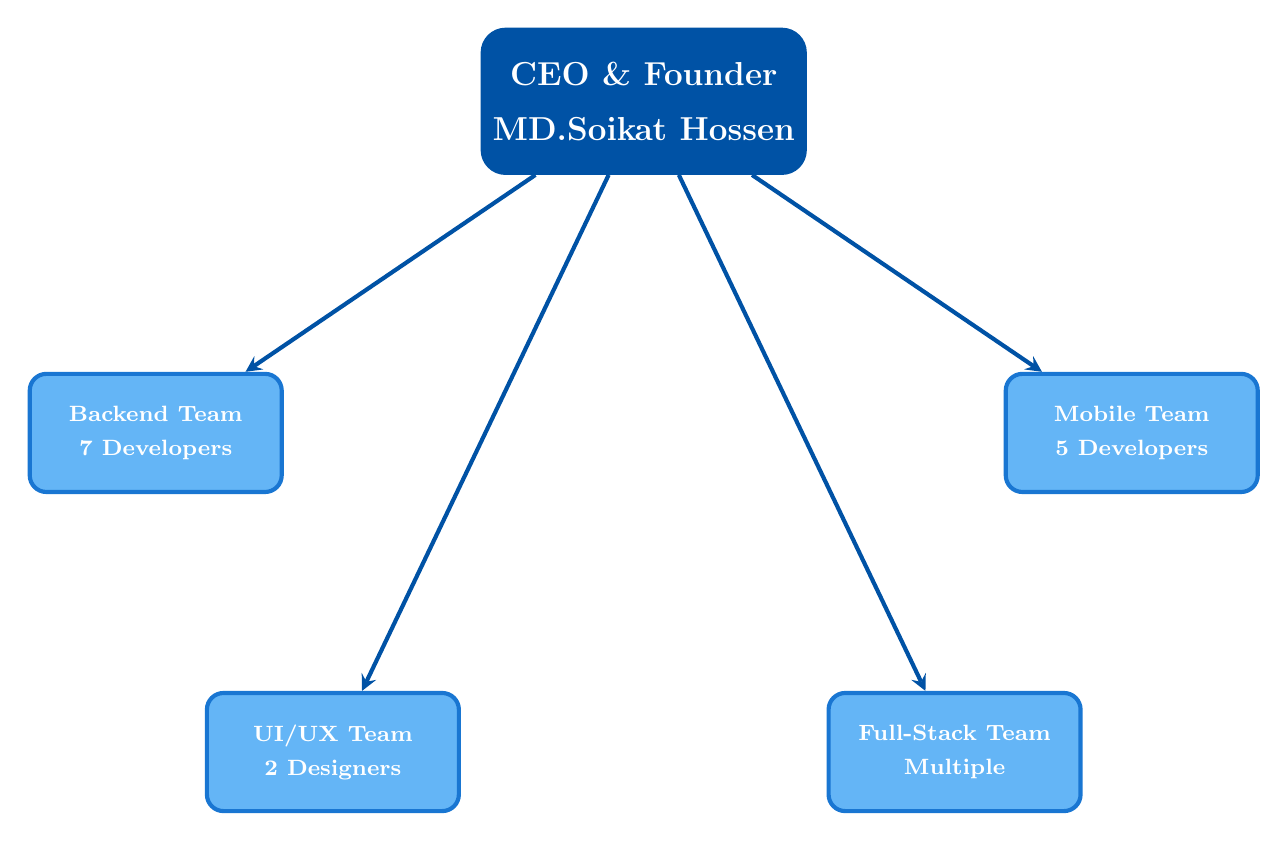
\begin{tikzpicture}[
        node distance=5cm and 4cm,
        ceo/.style={
            rectangle, 
            rounded corners=8pt, 
            minimum width=4cm, 
            minimum height=1.8cm, 
            text centered, 
            draw=primaryblue, 
            line width=2pt,
            fill=primaryblue,
            text=white,
            font=\large\bfseries, 
            align=center
        },
        team/.style={
            rectangle, 
            rounded corners=6pt, 
            minimum width=3.2cm, 
            minimum height=1.5cm, 
            text centered, 
            draw=secondaryblue, 
            line width=1.5pt,
            fill=accentblue,
            text=white,
            font=\footnotesize\bfseries, 
            align=center
        },
        arrow/.style={
            thick,
            ->,
            >=stealth,
            color=primaryblue,
            line width=1.5pt
        }
    ]
    
    % CEO at the top center
    \node[ceo] (ceo) {CEO \& Founder\\[0.2cm]MD.Soikat Hossen};
    
    % Teams arranged in a 2x2 grid below CEO with professional spacing
    \node[team, below left=2.5cm and 2.5cm of ceo] (backend) {Backend Team\\[0.1cm]7 Developers};
    \node[team, below right=2.5cm and 2.5cm of ceo] (mobile) {Mobile Team\\[0.1cm]5 Developers};
    \node[team, below=2.5cm of backend, xshift=2.25cm] (uiux) {UI/UX Team\\[0.1cm]2 Designers};
    \node[team, below=2.5cm of mobile, xshift=-2.25cm] (fullstack) {Full-Stack Team\\[0.1cm]Multiple};
    
    % Draw connection arrows
    \draw[arrow] (ceo) -- (backend);
    \draw[arrow] (ceo) -- (mobile);
    \draw[arrow] (ceo) -- (uiux);
    \draw[arrow] (ceo) -- (fullstack);
    
    \end{tikzpicture}
    }
    \vspace{0.3cm}
    \caption{Code Studio Organizational Structure}
    \label{fig:org_structure}
\end{figure}

\subsubsection{Detailed Organizational Hierarchy}
The Code Studio organizational structure consists of:

\begin{itemize}
    \item \textbf{CEO \& Founder (MD.Soikat Hossen)}
    \begin{itemize}
        \item Handles most important tasks including marketing, accounting, and project handling
        \item Manages overall business strategy and client relationships
        \item Oversees all 15 team members across different specializations
        \item Focuses on scaling the company to become fully remote in the future
    \end{itemize}
    
    \item \textbf{Backend Development Team (7 Developers)}
    \begin{itemize}
        \item Specializes in Node.js development
        \item Manages database operations using SQL and MySQL
        \item Handles server-side logic and API development
        \item Ensures system scalability and performance optimization
    \end{itemize}
    
    \item \textbf{Mobile App Development Team (5 Developers)}
    \begin{itemize}
        \item Expert in Google Flutter framework
        \item Develops cross-platform applications for both Android and iOS
        \item Focuses on creating new idea-based apps based on user needs
        \item Handles mobile-specific optimization and performance
    \end{itemize}
    
    \item \textbf{UI/UX Design Team (2 Designers)}
    \begin{itemize}
        \item Creates visually appealing and user-friendly interfaces
        \item Uses Figma for design and prototyping
        \item Ensures intuitive user experiences across all platforms
        \item Collaborates with development teams on implementation
    \end{itemize}
    
    \item \textbf{Full-Stack Developers}
    \begin{itemize}
        \item Handle both frontend (React, Next.js) and backend development
        \item Provide comprehensive solutions for complex projects
        \item Bridge the gap between different development teams
        \item Adapt to various project requirements and technologies
    \end{itemize}
\end{itemize}

\subsubsection{Communication and Workflow}
\begin{itemize}
    \item \textbf{Team Communication:} Google Meet for all team coordination
    \item \textbf{Project Flow:} Customer Requirements → UI/UX Designer → (Mobile App / Website) → Frontend/Backend Development
    \item \textbf{Testing Methodology:} Agile method with client-assisted testing
    \item \textbf{Project Capacity:} Handling 20+ concurrent projects out of 50+ total projects
\end{itemize}

\subsection{Recommendations}

Based on Code Studio's organizational analysis, the following strategic recommendations are proposed:

\begin{itemize}
    \item \textbf{Digital Marketing Enhancement:} Strengthen online presence through SEO optimization and social media engagement to expand global client base
    \item \textbf{Portfolio Diversification:} Explore emerging technologies (AI/ML integration, blockchain solutions) to maintain competitive advantage
    \item \textbf{Quality Assurance Standardization:} Implement automated testing frameworks to maintain 98.5\% success rate during scaling
    \item \textbf{Remote Infrastructure Development:} Establish robust cloud-based collaboration tools supporting distributed team operations
    \item \textbf{Client Relationship Management:} Deploy CRM systems for better project tracking and enhanced client communication efficiency
\end{itemize}

\subsection{Conclusion}

Code Studio demonstrates exceptional operational excellence with a remarkable 98.5% project success rate across 90+ completed projects since its establishment in 2018. The company's strategic evolution from "Code Art" to a comprehensive software development organization showcases effective growth management and market adaptation.

The 15-member specialized team structure, comprising 7 backend developers, 5 mobile app developers, and 2 UI/UX designers, utilizes a modern technology stack including React.js, Node.js, Flutter, and MySQL. This technical foundation enables cross-platform development capabilities and positions the company to handle diverse project requirements across multiple industry sectors including e-commerce, healthcare, education, and agriculture.

Code Studio's international presence, spanning from Bangladesh to the USA, combined with their commitment to remote operations, establishes a strong foundation for continued growth and global market expansion. Their systematic approach to client collaboration, quality assurance through agile methodologies, and focus on innovative solution development creates a competitive advantage in the rapidly evolving software development landscape.


\newpage
\pagestyle{chapter2style}

\section{Chapter 2: SDLC}


\subsection{Problem Identification}
Based on the interview conducted with Code Studio's CEO, several key problems and challenges have been identified that the company faces in its operations:

\subsubsection{Payment and Cash Flow Issues}
\begin{itemize}
    \item \textbf{Delayed Client Payments:} Sometimes clients don't pay the cost of the product on time, creating cash flow problems for the company
    \item \textbf{Impact on Operations:} Payment delays can affect the company's ability to pay employees and maintain operations
    \item \textbf{Historical Challenge:} The company once faced a complete shutdown for 15 days due to clients not paying on time and employees not working properly
\end{itemize}

\subsubsection{Project Management and Timeline Challenges}
\begin{itemize}
    \item \textbf{Unrealistic Client Expectations:} Some clients want the product delivered earlier than realistically possible, given that software development is time-consuming
    \item \textbf{Deadline Management:} The CEO identified that sometimes deadlines are not followed, which is considered the worst part of being a CEO
    \item \textbf{Quality vs. Speed Balance:} Maintaining the 98.5\% success rate while meeting tight deadlines poses ongoing challenges
\end{itemize}

\subsubsection{Operational and Growth Challenges}
\begin{itemize}
    \item \textbf{Remote Work Transition:} The company wants to operate fully remotely in the future, which requires significant operational changes
    \item \textbf{Team Management:} Managing a team of 15 employees across different specializations (5 mobile app developers, 7 backend developers, 2 UI/UX designers)
    \item \textbf{System Optimization:} The current product delivery system is not fully optimized according to the CEO's assessment
    \item \textbf{Website Issues:} The CEO wants to change the company website, indicating dissatisfaction with the current web presence
\end{itemize}

\subsubsection{Automation and Process Efficiency Challenges}
\begin{itemize}
    \item \textbf{Lack of Automated Project Management:} Manual tracking of 20+ concurrent projects leads to inefficiencies and potential oversight of critical milestones
    \item \textbf{Manual Client Communication:} Heavy reliance on manual WhatsApp and phone communications without automated notification systems
    \item \textbf{Absence of Automated Testing:} Limited automation in testing procedures, resulting in increased manual effort and potential human errors
    \item \textbf{Manual Resource Allocation:} Lack of automated systems for optimal team member assignment based on skills and availability
    \item \textbf{Manual Progress Monitoring:} No automated dashboard for real-time project progress tracking and performance analytics
    \item \textbf{Limited Automation in Deployment:} Manual deployment processes that could benefit from CI/CD automation pipelines
\end{itemize}

\subsection{Proposed Solutions}
Based on the identified problems, Code Studio has implemented or is considering the following solutions:

\begin{itemize}
    \item \textbf{Payment Solution:}
    \begin{itemize}
        \item Implement stricter payment terms and contracts
        \item Remove clients who consistently fail to pay on time
        \item Consider milestone-based payment structures
        \item Establish better financial management practices
    \end{itemize}
    
    \item \textbf{Project Management Solutions:}
    \begin{itemize}
        \item Better client education about realistic development timelines
        \item Implement agile methodology for better project tracking
        \item Use Google Meet for improved team communication
        \item Strengthen planning processes to avoid deadline issues
    \end{itemize}
    
    \item \textbf{Operational Solutions:}
    \begin{itemize}
        \item Gradual transition to remote work model
        \item Invest in employee training and development
        \item Optimize the product delivery system
        \item Redesign and improve the company website
        \item Focus on confident planning → increased marketing → more actions → increased product sales
    \end{itemize}

    \newpage
    \item \textbf{Comprehensive Automation System Solution:}
    \begin{itemize}
        \item \textbf{Integrated Project Management Platform:} Implement automated project tracking with real-time dashboards, milestone alerts, and progress monitoring
        \item \textbf{Smart Resource Allocation System:} AI-powered team assignment based on skills, availability, and project requirements
        \item \textbf{Automated Client Communication Hub:} Centralized notification system with automated status updates, milestone alerts, and progress reports
        \item \textbf{CI/CD Deployment Pipeline:} Automated testing, building, and deployment processes to reduce manual errors and accelerate delivery
        \item \textbf{Performance Analytics Dashboard:} Real-time monitoring of project KPIs, team productivity, and client satisfaction metrics
        \item \textbf{Automated Quality Assurance:} Integration of automated testing frameworks and code quality checks throughout the development lifecycle
    \end{itemize}
\end{itemize}

\subsection{Proposed Automation System Architecture}

\subsubsection{System Requirements}
The proposed automation system will address Code Studio's operational challenges through integrated modules:

\begin{itemize}
    \item \textbf{Core Platform Requirements:}
    \begin{itemize}
        \item Cloud-based infrastructure supporting 15+ concurrent users
        \item Real-time synchronization across global teams (Bangladesh and USA)
        \item Integration with existing tools (Google Meet, Figma, Postman)
        \item Mobile-responsive interface for remote team management
    \end{itemize}
    
    \item \textbf{Project Management Module:}
    \begin{itemize}
        \item Automated project creation from client requirements
        \item Task assignment based on team member expertise and availability
        \item Milestone tracking with automated alerts and notifications
        \item Resource allocation optimization for 20+ concurrent projects
    \end{itemize}
    
    \item \textbf{Communication Automation:}
    \begin{itemize}
        \item Automated client status updates via WhatsApp API integration
        \item Progress report generation and distribution
        \item Deadline reminders and escalation protocols
        \item Integrated team communication with Google Meet scheduling
    \end{itemize}
    
    \item \textbf{Quality Assurance Automation:}
    \begin{itemize}
        \item Automated testing pipeline for Flutter, React.js, and Node.js applications
        \item Code quality assessment and compliance checking
        \item Performance monitoring and optimization recommendations
        \item Automated deployment to testing and production environments
    \end{itemize}
\end{itemize}

\begin{figure}[H]
    \centering
    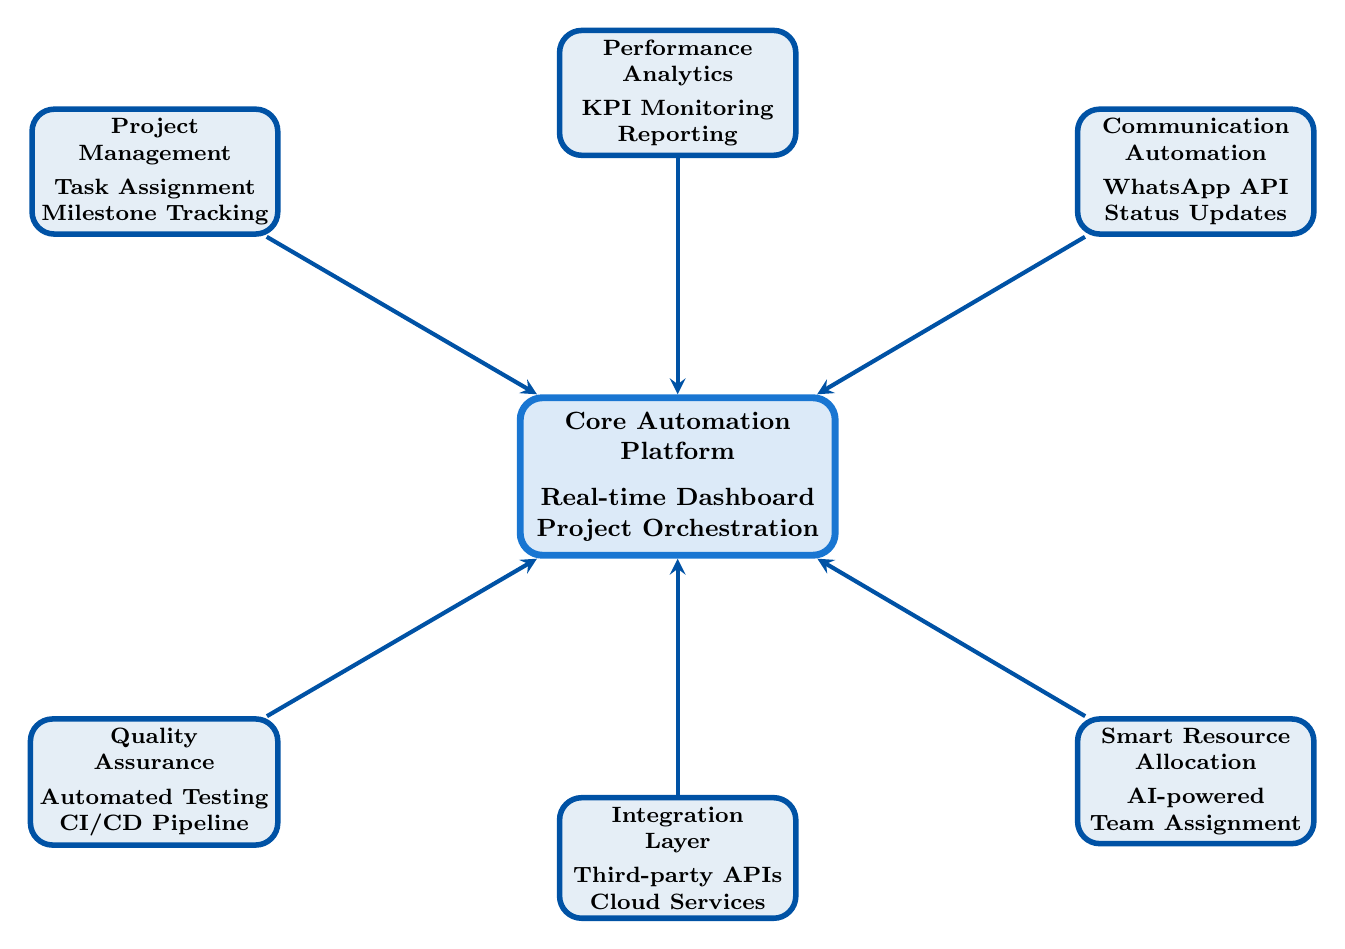
\begin{tikzpicture}[
        node distance=3cm and 4cm,
        component/.style={
            rectangle,
            rounded corners=8pt,
            minimum width=3cm,
            minimum height=1.5cm,
            text centered,
            draw=primaryblue,
            line width=2pt,
            fill=primaryblue!10,
            font=\footnotesize\bfseries,
            align=center
        },
        core/.style={
            rectangle,
            rounded corners=8pt,
            minimum width=4cm,
            minimum height=2cm,
            text centered,
            draw=secondaryblue,
            line width=2.5pt,
            fill=secondaryblue!15,
            font=\small\bfseries,
            align=center
        },
        arrow/.style={
            thick,
            ->,
            >=stealth,
            line width=1.5pt,
            color=primaryblue
        }
    ]
    
    % Core Automation Platform (center)
    \node[core] (core) at (0,0) {Core Automation\\Platform\\[0.2cm]Real-time Dashboard\\Project Orchestration};
    
    % Project Management Module (top left)
    \node[component, above left=2cm and 3cm of core] (pm) {Project\\Management\\[0.1cm]Task Assignment\\Milestone Tracking};
    
    % Communication Hub (top right)
    \node[component, above right=2cm and 3cm of core] (comm) {Communication\\Automation\\[0.1cm]WhatsApp API\\Status Updates};
    
    % Quality Assurance (bottom left)
    \node[component, below left=2cm and 3cm of core] (qa) {Quality\\Assurance\\[0.1cm]Automated Testing\\CI/CD Pipeline};
    
    % Resource Allocation (bottom right)
    \node[component, below right=2cm and 3cm of core] (resource) {Smart Resource\\Allocation\\[0.1cm]AI-powered\\Team Assignment};
    
    % Data Analytics (top center)
    \node[component, above=3cm of core] (analytics) {Performance\\Analytics\\[0.1cm]KPI Monitoring\\Reporting};
    
    % Integration Layer (bottom center)
    \node[component, below=3cm of core] (integration) {Integration\\Layer\\[0.1cm]Third-party APIs\\Cloud Services};
    
    % Arrows connecting components to core
    \draw[arrow] (pm) -- (core);
    \draw[arrow] (comm) -- (core);
    \draw[arrow] (qa) -- (core);
    \draw[arrow] (resource) -- (core);
    \draw[arrow] (analytics) -- (core);
    \draw[arrow] (integration) -- (core);
    
    \end{tikzpicture}
    \caption{Code Studio Automation Process Diagram}
    \label{fig:automation_process}
\end{figure}


\subsection{Automation System Feasibility Analysis}

This section provides a comprehensive feasibility analysis for implementing the proposed automation system at Code Studio, addressing technical, economic, operational, and schedule feasibility.

\subsubsection{Technical Feasibility Assessment}
\begin{itemize}
    \item \textbf{Infrastructure Requirements:}
    \begin{itemize}
        \item Cloud-based architecture compatible with existing AWS/Azure services
        \item Integration capabilities with current tech stack (React.js, Node.js, Flutter, MySQL)
        \item API compatibility for third-party service integrations (payment gateways, communication tools)
        \item Scalable microservices architecture supporting 50+ concurrent projects
    \end{itemize}
    
    \item \textbf{Technical Resources:}
    \begin{itemize}
        \item Current team expertise: 5 mobile developers, 7 backend developers, 2 UI/UX designers
        \item Existing development tools: Figma, Git, Postman already support automation workflows
        \item Database management capabilities with MySQL optimization experience
        \item High technical feasibility with minimal additional resource requirements
    \end{itemize}
    
    \item \textbf{System Integration:}
    \begin{itemize}
        \item Seamless integration with existing project management workflows
        \item Compatible with current communication channels (WhatsApp, email, Google Meet)
        \item Support for real-time collaboration and version control systems
        \item Automated testing and deployment pipeline integration
    \end{itemize}
\end{itemize}

\subsubsection{Economic Feasibility Analysis}
\begin{itemize}
    \item \textbf{Implementation Costs:}
    \begin{itemize}
        \item Initial software development and customization: ৳8,50,000 - ৳12,00,000
        \item Cloud infrastructure setup and configuration: ৳1,50,000 - ৳2,50,000
        \item Staff training and change management: ৳2,00,000 - ৳3,50,000
        \item Total initial investment: ৳12,00,000 - ৳18,00,000
    \end{itemize}
    
    \item \textbf{Operational Cost Savings:}
    \begin{itemize}
        \item Reduced manual project management time: 30\% efficiency gain
        \item Automated communication reduces coordination overhead by 25\%
        \item Quality assurance automation decreases testing time by 40\%
        \item Expected annual savings: ৳15,00,000 - ৳22,00,000
    \end{itemize}
    
    \item \textbf{Return on Investment:}
    \begin{itemize}
        \item ROI calculation: (Annual Savings - Implementation Cost) / Implementation Cost
        \item Projected ROI: 25-85\% in the first year
        \item Break-even point: 8-14 months after implementation
        \item Long-term benefits: Increased project capacity and client satisfaction
    \end{itemize}
\end{itemize}

\subsubsection{Operational Feasibility Evaluation}
\begin{itemize}
    \item \textbf{User Acceptance Analysis:}
    \begin{itemize}
        \item Team of 15 employees manageable for gradual system adoption
        \item Current use of digital tools (Google Meet, Figma) indicates high technology acceptance
        \item Management commitment to process improvement supports implementation
        \item Expected user adoption rate: 85-95\% within 3 months
    \end{itemize}
    
    \item \textbf{Process Integration:}
    \begin{itemize}
        \item Automation system designed to enhance existing 6-phase development process
        \item Minimal disruption to current client communication workflows
        \item Gradual implementation plan to maintain business continuity
        \item Enhanced quality metrics tracking and reporting capabilities
    \end{itemize}
    
    \item \textbf{Change Management Requirements:}
    \begin{itemize}
        \item Comprehensive training program for all team members
        \item Phase-wise implementation to minimize operational disruption
        \item Regular feedback collection and system optimization
        \item Support infrastructure for troubleshooting and maintenance
    \end{itemize}
\end{itemize}

\subsubsection{Schedule Feasibility Planning}
\begin{itemize}
    \item \textbf{Implementation Timeline:}
    \begin{itemize}
        \item Phase 1 - Core System Development: 8-10 weeks
        \item Phase 2 - Integration and Testing: 4-6 weeks
        \item Phase 3 - Training and Deployment: 3-4 weeks
        \item Phase 4 - Optimization and Fine-tuning: 2-3 weeks
        \item Total implementation time: 17-23 weeks (4-6 months)
    \end{itemize}
    
    \item \textbf{Risk Assessment and Mitigation:}
    \begin{itemize}
        \item Technical risks: Mitigated by experienced development team and phased approach
        \item Operational risks: Addressed through comprehensive training and gradual rollout
        \item Schedule risks: Buffer time included for testing and optimization phases
        \item Financial risks: Conservative cost estimates with contingency planning
    \end{itemize}
    
    \item \textbf{Success Metrics and Monitoring:}
    \begin{itemize}
        \item Project delivery time reduction: Target 25-30\% improvement
        \item Client satisfaction scores: Target increase from current levels
        \item Team productivity metrics: Measurement of task completion rates
        \item System uptime and reliability: Target 99.5\% availability
    \end{itemize}
\end{itemize}

\subsubsection{Feasibility Conclusion}
\begin{itemize}
    \item \textbf{Overall Assessment:} The automation system implementation shows across all evaluation criteria
    \item \textbf{Technical Viability:} Excellent compatibility with existing infrastructure and team expertise
    \item \textbf{Economic Justification:} Strong ROI potential with reasonable implementation costs
    \item \textbf{Operational Readiness:} Team and processes well-positioned for successful adoption
    \item \textbf{Strategic Alignment:} Automation system supports Code Studio's growth objectives and competitive positioning
    \item \textbf{Recommendation:} PROCEED with implementation following the proposed phased approach
\end{itemize}


\subsection{Recommendations}

Based on the SDLC analysis and feasibility study, the following strategic recommendations are proposed:

\begin{itemize}
    \item \textbf{Immediate Implementation:} Proceed with phased automation system deployment starting with financial management modules
    \item \textbf{Risk Mitigation:} Establish comprehensive backup protocols and disaster recovery procedures during system transition
    \item \textbf{Staff Development:} Conduct intensive training programs for team members on new automation tools and workflows
    \item \textbf{Performance Monitoring:} Deploy real-time analytics dashboards for continuous system optimization and quality assurance
    \item \textbf{Client Communication Enhancement:} Implement automated progress reporting and milestone notification systems
    \item \textbf{Scalability Planning:} Design modular architecture supporting future team expansion and international operations
\end{itemize}

\subsection{Conclusion}

Code Studio's comprehensive SDLC analysis reveals significant automation potential that can transform operational efficiency while maintaining their exceptional 98.5% project success rate. The proposed automation system offers substantial financial benefits with projected annual savings of ৳15,00,000-৳22,00,000 and an attractive ROI of 25-85% within the first year of implementation.

The feasibility study comprehensively validates the automation initiative across all critical dimensions. Technical feasibility is confirmed through compatibility with existing infrastructure and the team's strong expertise in React.js, Node.js, Flutter, and MySQL technologies. Economic justification is robust with reasonable implementation costs of ৳12,00,000-৳18,00,000 offset by substantial operational savings. Operational readiness is demonstrated by the team's current technology adoption and management's commitment to process improvement.

The strategic implementation roadmap provides a systematic approach to transformation, addressing key challenges including client payment delays, manual project tracking inefficiencies, and the need for enhanced remote operation capabilities. This framework positions Code Studio for sustainable growth while maintaining service quality and enabling successful transition to fully remote operations with international expansion capabilities.

\newpage
\pagestyle{chapter3style}

\section{Chapter 3: Information Gathering}

\subsection{Information Gathering}

Code Studio employs systematic interview techniques to gather comprehensive requirements and understand business operations. The information gathering process focuses on understanding organizational challenges, technological needs, and strategic objectives through structured interviews with key stakeholders.

\subsubsection{Interview Methodology}
\begin{itemize}
    \item \textbf{Primary Communication Channels:}
    \begin{itemize}
        \item WhatsApp consultation: +880 1784 286885 (24/7 availability)
        \item Direct phone interviews with Bangladesh and USA offices
        \item Email correspondence: codestudio4@gmail.com
        \item In-person meetings at Rajshahi office
    \end{itemize}
    
    \item \textbf{Interview Focus Areas:}
    \begin{itemize}
        \item Business operations and organizational structure
        \item Technical infrastructure and development processes
        \item Operational challenges and pain points
        \item Strategic objectives and growth plans
        \item Technology stack and tool utilization
    \end{itemize}
\end{itemize}

\subsubsection{Key Interview Questions and Answers}

The following represents a comprehensive interview session conducted with Code Studio's CEO to understand critical business aspects:
\vspace{0.3cm}

\textbf{Q1: Can you briefly describe is Code Studio and what it offers?}
\begin{itemize}
    \item \textbf{Answer:} Code Studio is mainly a software-based company that fully focuses on mobile app and website development. Especially, new idea-based apps are developed here depending on user needs and unique ideas that are shared. Apart from this, digital marketing, video editing, and graphic design are also included. It was established in 2018, inspired by other friends. The first name was Code Art.
\end{itemize}

\textbf{Q2: What are the company's mission and long-term strategic vision?}
\begin{itemize}
    \item \textbf{Answer:} There are currently 15 members working in this company. The CEO assured us and also added that he wants to operate his company fully remotely in the future and increase the team size. The CEO's main goal is to spread new ideas across the country to develop new innovations.
\end{itemize}

\textbf{Q3: What technology stack does Code Studio utilize?}
\begin{itemize}
    \item \textbf{Answer:} Mobile App Development uses Google Flutter (supports both Android and iOS). Website Development employs React and Next.js for frontend, Node.js for backend, and SQL/MySQL for database management.
\end{itemize}

\textbf{Q4: Can you describe the organizational structure and team composition?}
\begin{itemize}
    \item \textbf{Answer:} Currently, there are 15 employees. Soikat Bhai is the CEO and Founder who handles most important tasks like marketing, accounting, and project handling. More than 50 projects are involved, but around 20 projects are running at a time in Code Studio. Different types of employees work here, especially full-stack developers are hired more. There are 2 UI/UX designers, 5 mobile app developers, and 7 backend developers.
\end{itemize}

\textbf{Q5: How does Code Studio handle testing and quality assurance?}
\begin{itemize}
    \item \textbf{Answer:} Testing is done by clients, meaning the company helps the client fully to test the software. Follows the agile method. Only handles client projects, not other companies' tasks.
\end{itemize}

\textbf{Q6: What is the app building process at Code Studio?}
\begin{itemize}
    \item \textbf{Answer:} Customer Requirements → UI/UX Designer → two path split → Mobile App and Website → Frontend and Backend development.
\end{itemize}

\textbf{Q7: How does the team communicate and collaborate?}
\begin{itemize}
    \item \textbf{Answer:} Communication with team members is primarily through Google Meet for all coordination and meetings.
\end{itemize}

\textbf{Q8: How is financial management handled at Code Studio?}
\begin{itemize}
    \item \textbf{Answer:} The CEO handles financial management with great concern and personal oversight.
\end{itemize}

\textbf{Q9: What are the main operational challenges Code Studio faces?}
\begin{itemize}
    \item \textbf{Answer:} Sometimes clients don't pay the cost of the product on time. On the other hand, some clients want the product earlier, which is not always possible as it is time-consuming. These are the main problems faced by the CEO.
\end{itemize}

\textbf{Q10: What is Code Studio's main competitive strength?}
\begin{itemize}
    \item \textbf{Answer:} The employees' technical experience is our main strength.
\end{itemize}

\textbf{Q11: What is Code Studio's path to success?}
\begin{itemize}
    \item \textbf{Answer:} Confident planning → Increased marketing → More actions performed → Increased product sales. The company is always dynamic.
\end{itemize}

\textbf{Q12: What are Code Studio's primary goals?}
\begin{itemize}
    \item \textbf{Answer:} Less investment → More benefit. Focus on location, financial, and time freedom. The goal is to become a fully remote-based company.
\end{itemize}

\textbf{Q13: What major challenges has Code Studio overcome?}
\begin{itemize}
    \item \textbf{Answer:} Once, clients didn't pay on time and employees didn't work properly, so the company was fully stopped for 15 days. That was a big challenge. It was overcome technically through planning, such as removing some employees as well as clients who wouldn't pay. The team is now fully manageable.
\end{itemize}

\textbf{Q14: What is the best and worst part of being a CEO?}
\begin{itemize}
    \item \textbf{Answer:} Best part: Can handle employees technically. Worst part: Sometimes deadlines are not followed.
\end{itemize}

\textbf{Q15: What does the CEO want to change in the company?}
\begin{itemize}
    \item \textbf{Answer:} The company website needs improvement and updating.
\end{itemize}

\textbf{Additional Short Questions and Responses:}
\begin{itemize}
    \item \textbf{Q:} Do you believe Code Studio has the potential to expand internationally? \textbf{A:} Yes
    \item \textbf{Q:} Is customer satisfaction the top priority at Code Studio? \textbf{A:} Yes
    \item \textbf{Q:} Are you satisfied with the current growth rate of Code Studio? \textbf{A:} Yes
    \item \textbf{Q:} Does Code Studio invest enough in employee training and development? \textbf{A:} Yes
    \item \textbf{Q:} Is the current product delivery system at Code Studio fully optimized? \textbf{A:} No
\end{itemize}

\subsection{Interview Analysis}

The comprehensive interview with Code Studio's CEO provides valuable insights into the company's operational dynamics, strategic vision, and challenges. This analysis examines key themes emerging from the interview responses to understand the organization's current state and future trajectory.

\subsubsection{Organizational Strengths Assessment}

Based on the interview responses, Code Studio demonstrates several core organizational strengths:

\begin{itemize}
    \item \textbf{Technical Excellence and Team Expertise:} The CEO identified "employees' technical experience" as the company's main competitive strength. With 15 specialized team members including 7 backend developers, 5 mobile app developers, and 2 UI/UX designers, the company has built a robust technical foundation.
    
    \item \textbf{Modern Technology Stack:} Code Studio utilizes cutting-edge technologies including Google Flutter for cross-platform mobile development, React and Next.js for frontend development, Node.js for backend services, and SQL/MySQL for database management. This comprehensive technology stack enables the company to deliver end-to-end solutions.
    
    \item \textbf{Impressive Project Success Rate:} The company maintains a 98.5\% project success rate across 90+ completed projects, demonstrating exceptional quality control and client satisfaction capabilities.
    
    \item \textbf{Strategic Market Position:} With operations spanning from Bangladesh to the USA and successful collaboration with 25+ startup companies globally, Code Studio has established a strong international presence and market credibility.
\end{itemize}

\subsubsection{Leadership and Management Analysis}

The interview reveals CEO MD. Soikat Hossen's hands-on leadership approach and strategic thinking:

\begin{itemize}
    \item \textbf{Comprehensive Role Management:} The CEO handles critical functions including marketing, accounting, and project management, demonstrating deep involvement in all business aspects.
    
    \item \textbf{Strategic Vision for Remote Operations:} The clear goal to operate fully remotely in the future shows forward-thinking leadership aligned with global industry trends and post-pandemic work preferences.
    
    \item \textbf{Innovation Focus:} The CEO's goal to "spread new ideas across the country to develop new innovations" indicates a commitment to technological advancement and market development.
    
    \item \textbf{Honest Self-Assessment:} The CEO's acknowledgment that "sometimes deadlines are not followed" as the worst part of being a CEO shows transparency and awareness of areas needing improvement.
\end{itemize}

\subsubsection{Operational Challenges Identification}

The interview identified several critical operational challenges requiring strategic attention:

\begin{itemize}
    \item \textbf{Payment and Cash Flow Management:} Client payment delays represent a significant operational risk, historically causing a 15-day complete shutdown. This challenge directly impacts the company's ability to maintain operations and pay employees.
    
    \item \textbf{Client Expectation Management:} Unrealistic client timeline expectations create pressure on project delivery, potentially affecting quality standards and team morale.
    
    \item \textbf{System Optimization Needs:} The CEO's admission that "the current product delivery system is not fully optimized" indicates significant room for process improvement and efficiency gains.
    
    \item \textbf{Digital Presence Concerns:} The desire to change the company website suggests current digital marketing and brand presentation may not meet the CEO's standards for business growth.
\end{itemize}

\subsection{Information Integration}

The information gathering process reveals Code Studio as a technologically advanced organization with strong fundamentals but facing growth-related challenges. Integration of interview data provides a comprehensive understanding of the company's operational ecosystem.

\subsubsection{Business Model Analysis}

Code Studio operates on a client-focused software development model with the following characteristics:

\begin{itemize}
    \item \textbf{Service Portfolio:} Comprehensive software development services including mobile applications, web development, UI/UX design, digital marketing, video editing, and graphic design.
    
    \item \textbf{Development Methodology:} Structured workflow following Customer Requirements → UI/UX Design → Mobile App/Website Development → Frontend/Backend Implementation, supported by agile methodology and client-assisted testing.
    
    \item \textbf{Quality Assurance Approach:} Client-collaborative testing methodology ensuring user requirements are met while maintaining the impressive 98.5\%.
    
    \item \textbf{Communication Infrastructure:} Google Meet-based team coordination with multi-channel client communication including WhatsApp (+880 1784 286885), email (codestudio4@gmail.com), and direct phone support.
\end{itemize}

\subsubsection{Technology Infrastructure Assessment}

The interview reveals a robust technology infrastructure supporting diverse development requirements:

\begin{itemize}
    \item \textbf{Cross-Platform Mobile Development:} Google Flutter framework enabling simultaneous Android and iOS application development, reducing development time and costs.
    
    \item \textbf{Modern Web Development Stack:} React and Next.js frontend technologies combined with Node.js backend services provide scalable, maintainable web applications.
    
    \item \textbf{Database Management:} SQL/MySQL database systems supporting complex data requirements across multiple concurrent projects.
    
    \item \textbf{Development Tools Integration:} Utilization of industry-standard tools including Figma for design, Git for version control, and Postman for API testing.
\end{itemize}

\subsubsection{Strategic Growth Framework}

The CEO outlined a clear strategic approach to business growth and success:

\begin{itemize}
    \item \textbf{Growth Strategy:} "Confident planning → Increased marketing → More actions performed → Increased product sales" demonstrates a systematic approach to business expansion.
    
    \item \textbf{Operational Philosophy:} "Less investment → More benefit" with focus on "location, financial, and time freedom" indicates efficiency-focused operations and remote work preparation.
    
    \item \textbf{Market Expansion Goals:} International expansion potential confirmed by CEO, supported by existing USA operations and global startup collaborations.
    
    \item \textbf{Innovation Commitment:} Emphasis on developing "new idea-based apps" based on user needs demonstrates market-responsive innovation capabilities.
\end{itemize}

\subsection{Recommendations}

Based on the comprehensive interview analysis and information integration, the following strategic recommendations address Code Studio's identified challenges while leveraging organizational strengths:

\subsubsection{Financial Management and Payment System Enhancement}

\begin{itemize}
    \item \textbf{Automated Payment Tracking System:} Implement digital invoicing and payment reminder systems to reduce manual oversight and ensure timely client payments.
    
    \item \textbf{Milestone-Based Payment Structure:} Establish project milestone-based payment schedules with contractual penalties for delayed payments to maintain steady cash flow.
    
    \item \textbf{Client Financial Screening:} Develop client vetting procedures to assess payment reliability before project initiation, reducing financial risks.
    
    \item \textbf{Emergency Cash Flow Management:} Establish financial reserves and backup funding sources to prevent operational shutdowns during payment delays.
\end{itemize}

\subsubsection{Process Optimization and System Enhancement}

\begin{itemize}
    \item \textbf{Project Management Automation:} Deploy integrated project management platforms with real-time tracking, automated milestone alerts, and progress monitoring for the 20+ concurrent projects.
    
    \item \textbf{Client Communication Automation:} Implement automated status update systems via WhatsApp API integration and email notifications to improve client engagement and reduce manual communication overhead.
    
    \item \textbf{Quality Assurance Standardization:} Establish automated testing frameworks and code quality checks to maintain the 98.5% success rate while reducing manual testing time.
    
    \item \textbf{Resource Allocation Optimization:} Create AI-powered team assignment systems based on developer skills, availability, and project requirements to maximize efficiency.
\end{itemize}

\subsubsection{Remote Operations and Team Management}

\begin{itemize}
    \item \textbf{Remote Infrastructure Development:} Invest in cloud-based collaboration tools, secure VPN systems, and virtual project management platforms to support the CEO's vision of fully remote operations.
    
    \item \textbf{Team Communication Enhancement:} Expand beyond Google Meet to include integrated communication platforms with file sharing, project tracking, and team coordination capabilities.
    
    \item \textbf{Performance Monitoring Systems:} Implement remote team productivity tracking and performance analytics to maintain quality standards in distributed work environments.
    
    \item \textbf{Digital Training Programs:} Develop online training modules for team skill development and technology updates to support continuous improvement.
\end{itemize}

\subsubsection{Digital Presence and Marketing Enhancement}

\begin{itemize}
    \item \textbf{Website Redesign and Optimization:} Address the CEO's concern by implementing a modern, SEO-optimized website showcasing the company's portfolio, technology stack, and success stories.
    
    \item \textbf{Digital Marketing Strategy:} Develop comprehensive online marketing campaigns leveraging social media, content marketing, and search engine optimization to expand global client base.
    
    \item \textbf{Portfolio Showcase Platform:} Create interactive portfolio sections highlighting successful projects like S-Finder, Grameen School, and Banglar Train applications.
    
    \item \textbf{Client Testimonial Integration:} Implement client feedback systems and testimonial displays to leverage the 98.5\% success rate for marketing purposes.
\end{itemize}

\subsection{Conclusion}

The comprehensive information gathering process through structured interviews with Code Studio's CEO has provided valuable insights into a technically proficient organization with strong market positioning and clear growth potential. The company demonstrates exceptional operational capabilities with a 98.5\% project success rate, modern technology stack implementation, and successful international collaborations with 25+ startup companies globally.

The interview analysis reveals MD. Soikat Hossen's strategic leadership approach, emphasizing technical excellence, innovation, and remote operations vision. The identification of critical challenges including payment management issues, process optimization needs, and system enhancement requirements provides clear direction for organizational improvement while maintaining competitive advantages.

Code Studio's strong technical foundation, comprising 15 specialized team members with expertise in Flutter, React.js, Node.js, and MySQL technologies, positions the company well for implementing recommended improvements. The systematic approach to project management, agile methodology adoption, and client-collaborative testing demonstrates mature operational practices that can be enhanced through targeted automation and process optimization.

The strategic recommendations addressing financial management enhancement, process automation, remote operations infrastructure, and digital presence improvement create a comprehensive roadmap for sustainable growth. These improvements will support the CEO's vision of fully remote operations while maintaining the company's impressive success rate and enabling international market expansion.

The information integration confirms Code Studio as a dynamic, technology-forward organization with the foundational strength necessary for continued growth and market leadership in the competitive software development industry. The company's commitment to innovation, quality excellence, and client satisfaction establishes a solid platform for implementing strategic improvements and achieving long-term business objectives.

\end{document}
